\chapter{Results} % Main chapter title

\label{Chapter 4} % Change X to a consecutive number; for referencing this chapter elsewhere, use \ref{ChapterX}

%-----------------------------------
%	SECTION 1
%-----------------------------------
\section{Accuracy Comparison of Regular Networks}


In order to evaluate the relative performance of each network over time, we measured classification accuracy on the test set at periodic intervals during training. We calculated the accuracy every X training images for the first Y images and every Z image thereafter, and final classification accuracy was measured after training was complete.

Results for the regular sized networks are shown in Figure [X]. Both LeNet and BackPanNet quickly achieve good classification rates, with a final accuracy of 98.68\% for LeNet and 98.94\% for backPanNet. (The reported final accuracy for LeNet in [cite] is X, which is reassuringly close to our value.) LeNet initially outperformed backPanNet, but backPanNet had a slight advantage after approximately X training images.

Our network of interest, PanNet, did not perform as well here. It achieved a final accuracy of 93.32\%. However, it may be that PanNet's performance would improve with additional training. 

A sample of the filters each network learned are shown in figure X [I don't think you have this figure in the paper just yet, but can you add it easily?]

To visualize the role each filter played, we calculated the activation of each pixel location for each filter, averaged across 1000 [is this right?] test images. This showed us the regions of the images where the filters tended to be activated. In PanNet, each filter was used in most areas of the images, whereas the backpropagation training in LeNet and backPanNet allowed the networks to create more refined filters that were only active in specific regions.



\begin{figure}[t!]
    \centering
    \begin{subfigure}[t]{0.3\textwidth}
        \centering
        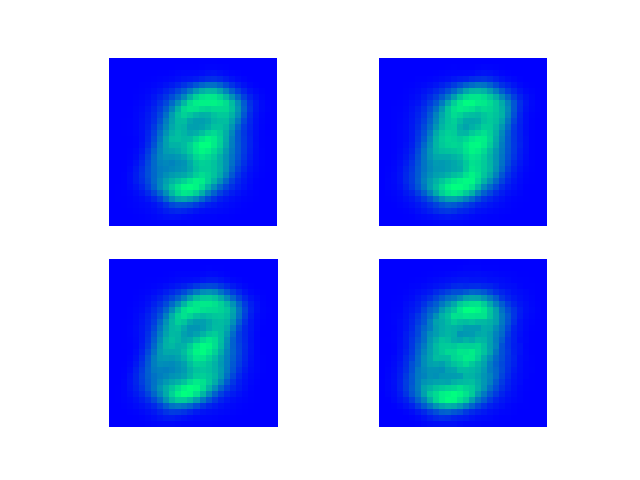
\includegraphics[height=1.2in]{Figures/PanNet}
        \caption{PanNet}
    \end{subfigure}
    \begin{subfigure}[t]{0.3\textwidth}
        \centering
        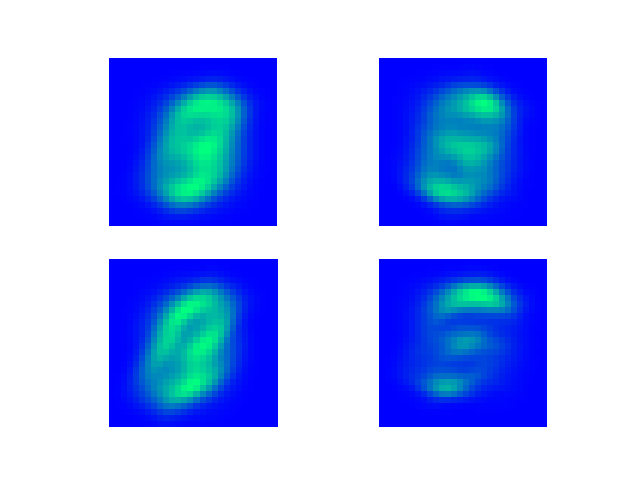
\includegraphics[height=1.2in]{Figures/backPanNet}
        \caption{backPanNet}
    \end{subfigure}%
    \begin{subfigure}[t]{0.3\textwidth}
        \centering
        \includegraphics[height=1.2in]{Figures/Lenet}
        \caption{LeNet}
    \end{subfigure}%
    \caption{\\Input activation area of each filter for PanNet,  backPanNet, and LeNet-1}
\end{figure}


[Change other figures in the paper, where necessary, to use the subfigure structure shown above, so that you can give captions to the individual subfigures]

[Remove the below paragraphs]
In figure \ref{fig:net_accu_plot_combined}, accuracy is calculated using testing set. Accuracy is calculated every 10 batches before 1,000 batches and every 1,000 batches after the first 1,000 batches. 

As can be seen from figure \ref{fig:net_accu_plot_combined}, LeNet-1 performs better than backPanNet in the first 1,000 batches but backPanNet outperforms LeNet-1 after 10,000 batches. The final accuracy for LeNet-1 is 98.68\% and the one for backPanNet is 98.94\%. PanNet performs worst among regular networks with a final accuracy of 93.32\%. 

\begin{figure}[th]
\centering
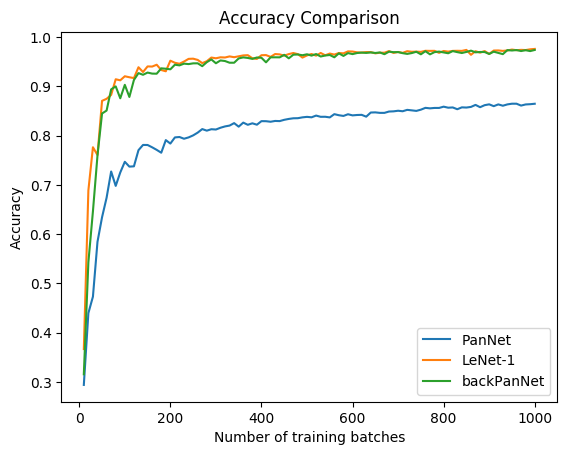
\includegraphics[width=65mm]{Figures/net_accu_plot_combined_1}
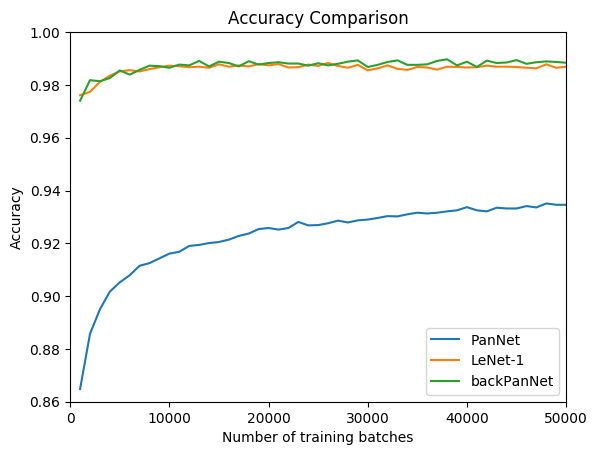
\includegraphics[width=65mm]{Figures/net_accu_plot_combined_2}
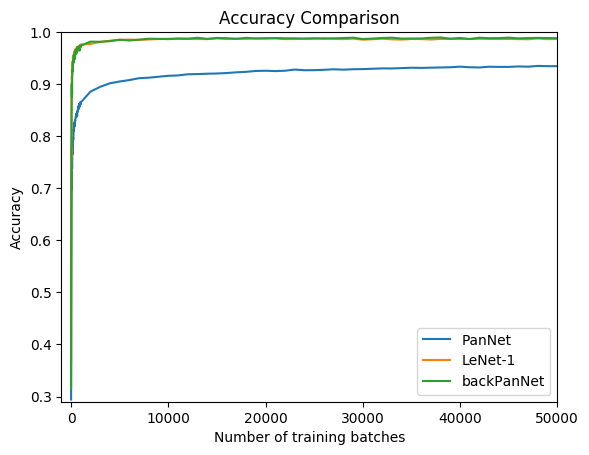
\includegraphics[width=65mm]{Figures/net_accu_plot_combined}
\decoRule
\caption{\\Accuracy versus number of training batches for regular networks}
\label{fig:net_accu_plot_combined}
\end{figure}

%-----------------------------------
%	SECTION 2
%-----------------------------------
\section{Accuracy Comparison of Enlarged Networks}

We speculated that the relatively poor performance of PanNet was due to the small number of filters in layer X. These filters were optimized through autoencoder learning to retain the information necessary to reconstruct their inputs, but in doing so they may have been trained to discard information that would eventually have been helpful in the final classification task. We thought that with more filters, the network would have more capacity to retain information that was marginally helpful in the reconstruction task but more helpful to classification. In order to fairly compare the different architectures, we also created enlarged versions of backPanNet and LeNet with more filters.

As with the regular-sized networks, backPanNet and LeNet still performed best, achieving final accuracies of 99.16\% and 99.22\%, respectively. Interestingly, here backPanNet initially took the lead and was eventually overtaken by LeNet, the reverse of the situation with the regular networks. It seems that the initial autoencoder training created filters that were close to the final versions, so that the final training was very fast. After only X training images, backPanNet already had an accuracy of 54.42\%!

PanNet performed quite respectably in the enlarged networks, with a final accuracy of 97.21\%, although it took many training examples to reach this value.

We examined the filter response plots for the enlarged networks, as can be seen from figure \ref{fig:filters_enlarged}. Here, plots look alike for all three architectures. With more available filters, even PanNet was able to learn dedicated filters which only responded to the very specific region (eg. a line). 

Finally, we examined the role of learning rate in the PanNet network, to see whether a different late would allow the network to more quickly achieve optimal performance. As seen in Figure \ref{fig:enlarged_net_accu_plot_combined_lr}, the optimal learning rate was 0.01, leading to a final accuracy of 97.65\%. However, since this was close to the accuracy achieved with the rate 0.1, which we used for the other networks, we stayed with 0.1 for the rest of the work.



\begin{figure}[th]
\centering
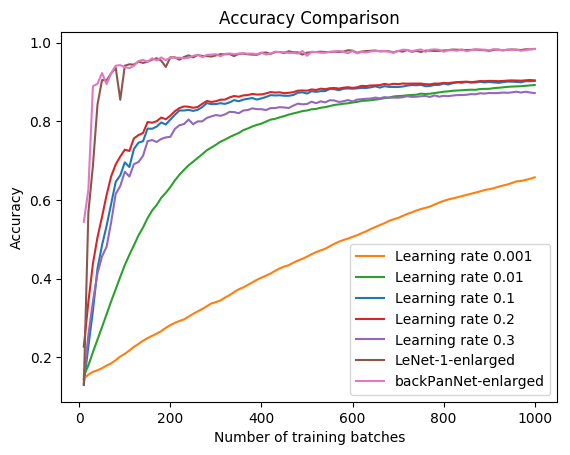
\includegraphics[width=65mm]{Figures/enlarged_net_accu_plot_combined_lr_1}
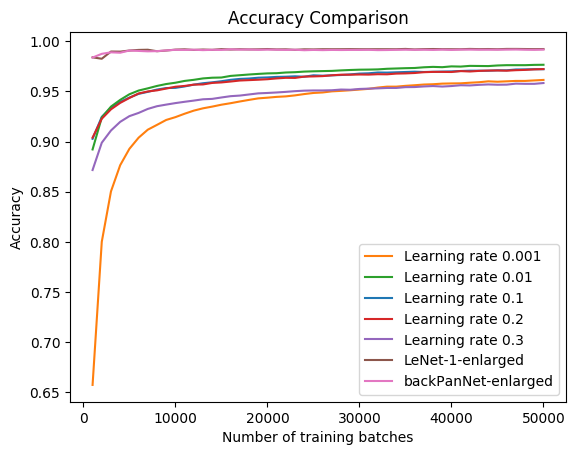
\includegraphics[width=65mm]{Figures/enlarged_net_accu_plot_combined_lr_2}
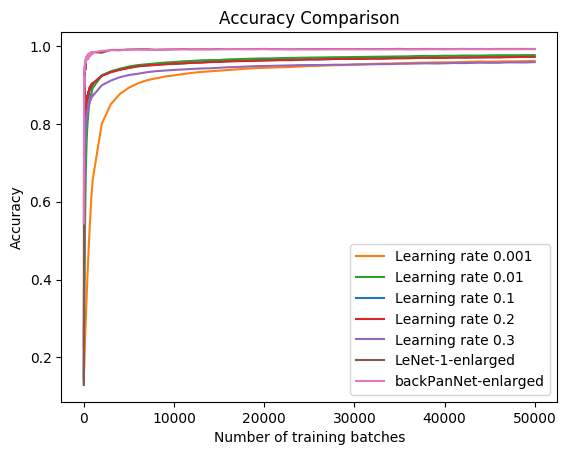
\includegraphics[width=65mm]{Figures/enlarged_net_accu_plot_combined_lr}
\decoRule
\caption{\\Accuracy versus number of training batches for enlarged networks}
\label{fig:enlarged_net_accu_plot_combined_lr}
\end{figure}



The final accuracy results for all the architectures are summarized in Table \ref{tab:summary_acc}.  

\begin{figure}[th]
\centering
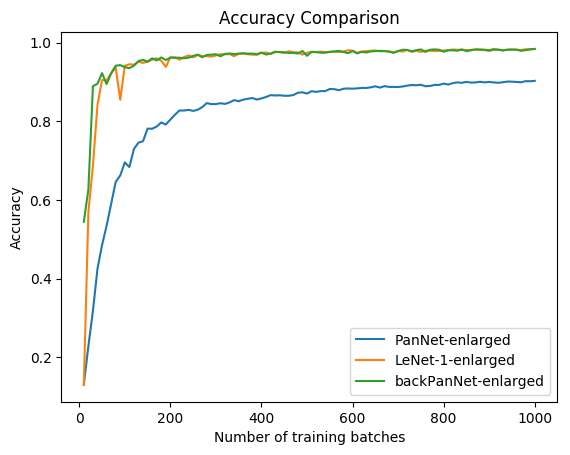
\includegraphics[width=65mm]{Figures/enlarged_net_accu_plot_combined_1}
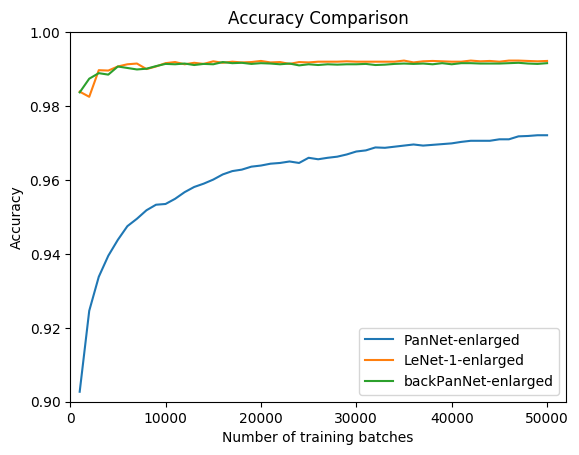
\includegraphics[width=65mm]{Figures/enlarged_net_accu_plot_combined_2}
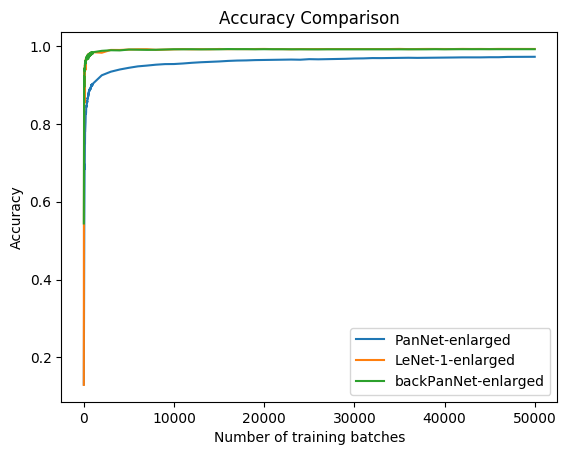
\includegraphics[width=65mm]{Figures/enlarged_net_accu_plot_combined}
\decoRule
\caption{\\Accuracy versus number of training batches for enlarged networks}
\label{fig:enlarged_net_accu_plot_combined}
\end{figure}




\begin{figure}[th]
\centering
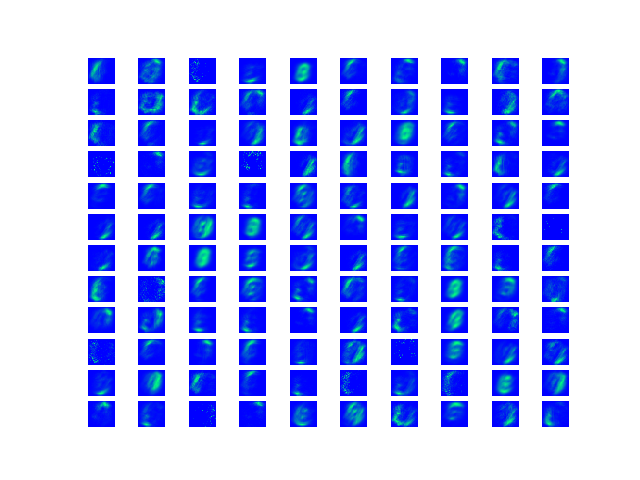
\includegraphics[width=95mm]{Figures/PanNet-enlarged}
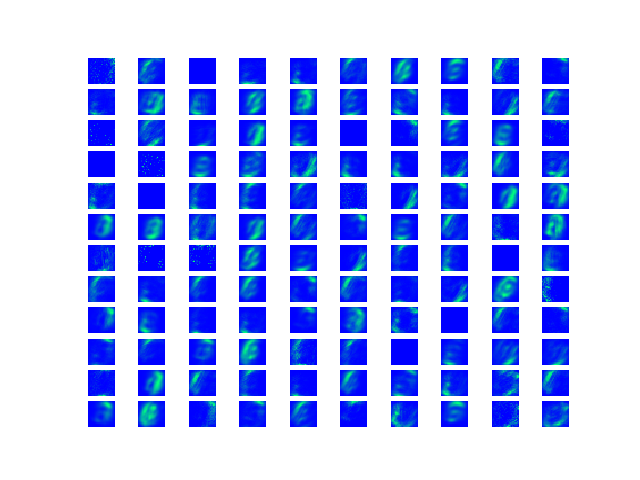
\includegraphics[width=95mm]{Figures/LeNet-enlarged}
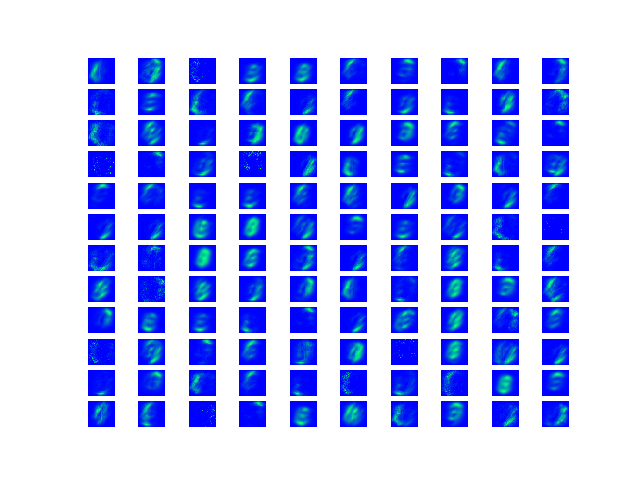
\includegraphics[width=95mm]{Figures/backPanNet-enlarged}
\decoRule
\caption{\\Input activation area of each filter for PanNet-enlarged, LeNet-1-enlarged and backPanNet-enlarged}
\label{fig:filters_enlarged}
\end{figure}



\begin{table}
\centering
\caption{Summary of all neural networks}\label{tab:summary_acc}
\begin{tabular}{l c c c c c c}
\toprule
& PanNet & \makecell{PanNet\\-enlarged}& LeNet-1 & \makecell{LeNet-1\\-enlarged}  & backPanNet & \makecell{backPanNet\\-enlarged}\\
\midrule
\makecell{Final \\ accuracy} & 93.32\% & \makecell{97.21\% \\ 97.65\% when \\ learning \\ rate is 0.01} & 98.68\% & \textbf{99.22}\% & 98.94\% & 99.16\%\\ 
\bottomrule\\
\end{tabular}
\end{table}
